\documentclass{article}
\usepackage[utf8]{inputenc}
\usepackage[a4paper, total={6in, 8in}]{geometry}
\usepackage{amsmath}
\usepackage{bm}
\usepackage{xcolor}
%\usepackage{epstopdf}
\usepackage{graphicx}
\usepackage{upgreek}
\usepackage[style=numeric]{biblatex}
\addbibresource{bibliography.bib}

\title{Jagadeeshan Group Single-Chain Code Documentation}
\author{Isaac Pincus}
\date{Last compiled: \today}

\begin{document}

\maketitle

\tableofcontents

\section{Introduction}
This document will detail the theory behind the single-chain BD code.
The key equations are listed here in the introduction, with separate sections for each of the additional features.
Currently, this code includes the following BD features:

\begin{itemize}
    \item Semi-implicit predictor-corrector BD algorithm
    \item Hydrodynamic interaction mediated by Rotne-Prager-Yamakawa (RPY) tensor, with decomposition using Fixman's method
    \item Excluded volume interactions of Gaussian, Lennard-Jones or SDK form
    \item A variety of spring potentials, including Hookean, FENE, Fraenkel, MS-WLC, FENE-Fraenkel and inverse Langevin with the Pade approximation.
    \item Bending potential of arbitrary form
    \item Form of solvent velocity field can be specified, and set arbitrarily
\end{itemize}

\subsection{Algorithm Overview}
The algorithm predominately follows Prabhakar and Prakash \cite{Prabhakar2004}, who detail a semi-implicit predictor-corrector scheme with hydrodynamic interaction and excluded volume.
This algorithm is for a linear bead-spring chain of $N$ massless beads at positions $\{\bm{r}_\nu | \nu=1,\dots,N\}$, suspended in an incompressible Newtonian solvent with velocity field $\bm{v} = \bm{v}_0 + \bm{\kappa} \cdot \bm{r}$, where $\bm{\kappa}=(\nabla \bm{v})^{\mathrm{T}}$ is independent of position.
The bead positions follow a probability distribution function $\psi\left(\bm{r}_{1}, \ldots, \bm{r}_{N}\right)$.
This can be shown to give the following Fokker-Planck equation \cite{Bird1987}:
\begin{equation}
\label{Fokker-Planck equation}
    \frac{\partial \psi^{*}}{\partial t^{*}}=-\sum_{\nu=1}^{N} \frac{\partial}{\partial \bm{r}_{\nu}^{*}} \cdot\left\{\bm{\kappa}^{*} \cdot \bm{r}_{\nu}^{*}+\frac{1}{4} \sum_{\mu} \bm{\Upsilon}_{\nu \mu} \cdot \bm{F}_{\mu}^{\phi *}\right\} \psi^{*}+\frac{1}{4} \sum_{\nu, \mu=1}^{N} \frac{\partial}{\partial \bm{r}_{\nu}^{*}} \cdot \bm{\Upsilon}_{\nu \mu} \cdot \frac{\partial \psi^{*}}{\partial \bm{r}_{\mu}^{*}}
\end{equation}
where variables have been scaled in terms of characteristic length scale $l_H = \sqrt{k_\mathrm{B} T}$ and characteristic time scale $\lambda_H = \zeta/4H$, where $k_\mathrm{B}$ is the Boltzmann's constant, $T$ is the absolute temperature, $H$ is the Hookean spring stiffness constant, and $\zeta$ is the Stokesian bead-friction parameter, which for a bead with hydrodynamic radius $a$ in a solvent of viscosity $\eta_s$ is given by $\zeta = 6 \pi a \eta_s$.
This choice of non-dimensionalisation necessitates the spring force law to be written in the form:
\begin{equation}
    \bm{F}^{c}_\nu = H \bm{Q}_\nu f(Q)
\end{equation}
where $\bm{Q}_\nu = \bm{r}_{\nu+1} - \bm{r}_\nu$ is the bead-bead connector vector, $\bm{F}^{c}_\nu$ is the tension in the spring $\nu$ (such that the net spring force on bead $\nu$ is $\bm{F}^{S}_\nu = \bm{F}^{c}_\nu - \bm{F}^{c}_{\nu-1}$), and $f(Q)$ is some dimensionless function of the connector vector length $Q$. 
The hydrodynamic interactions along the chain length are taken into account by the dimensionless tensor $\bm{\Upsilon}_{\nu \mu} = \delta_{\nu \mu} \bm{\delta} + \zeta \bm{\Omega}_{\nu \mu}$, where $\delta_{\nu \mu}$ is the Kronecker delta, $\bm{\delta}$ is the unit tensor and $\bm{\Omega}$ is a tensor representing the hydrodynamic interaction between the beads $\nu$ and $\mu$.
Finally, the force $\bm{F}_{\mu}^{\phi *}$ represents all conservative forces acting on each bead $\mu$, for example from the connector vector spring force, excluded volume interactions, and bending potential.

The numerical integration of Eq.~\eqref{Fokker-Planck equation} is undertaken on the basis of the equivalent It\^{o} stochastic differential equation for the chain configuration, which is given by Prabhakar and Prakash as:
\begin{equation}
\label{Ito SDE}
    \mathrm{d} \bm{R}=\left[\bm{K} \cdot \bm{R}+\frac{1}{4} \bm{D} \cdot \bm{F}^{\phi}\right] \mathrm{d} t^{*}+\frac{1}{\sqrt{2}} \bm{B} \cdot \mathrm{d} \bm{W}
\end{equation}
where $\bm{R}$ is a $3\times N$ matrix containing bead co-ordinates, $\bm{K}$ is a $3N \times 3N$ block matrix with the diagonal blocks containing $\bm{\kappa}^*$ and others euqal to 0, $\bm{F}^{\phi}$ is a $3 \times N$ matrix containing total force vectors on each bead, $\bm{D}$ is a $3N \times 3N$ block matrix where the $\nu \mu$ block contains the $\bm{\Upsilon}_{\nu \mu}$ tensor components, $\bm{W}$ is a $3\times N$ dimensional Wiener process and $\bm{B}$ is a matrix such that $\bm{D} = \bm{B} \cdot \bm{B}^{\mathrm{T}}$.
Note that this structure is very similar to the actual data structure used in our implementation, except that $\bm{K} \cdot \bm{R}$ is simply the $3\times 3$ matrix $\bm{\kappa}^*$ matrix-multiplied by the $3\times N$ matrix $\bm{R}$, and the diffusion matrix $\bm{D}$ is actually a $3 \times N \times 3 \times N$ 4-D array, which if imagined as an $N\times N$ block matrix of $3\times 3$ $\bm{\Upsilon}_{\nu \mu}$ tensors, only has the upper diagonal elements filled in (as in, it is 0 for $\nu > \mu$). 

The key solution algorithm in the procedure Time\_Integrate\_Chain then proceeds as follows for each timestep of the simulation:
\begin{itemize}
    \item The bead positions are moved by a constant factor such that the center of mass is at $(0,0,0)$. 
    \item The bead-to-bead vectors and distances are calculated and placed into two $3 \times N \times N$ and $N \times N$ superdiagonal matrices.
    \item The spring force (section link), excluded volume force (section link) and bending potential (section link) are all calculated.
    \item The bead-bead diffusion tensors making up the matrix $\bm{D}$ are calculated (section link)
    \item Samples are taken to store bead trajectories and calculate material functions (section link)
    \item The value of $\bm{B} \cdot \mathrm{d} \bm{W}$ for the timestep is calculated using Chebyshev polynomial approximation as per Fixman (citation and section link)
    \item The semi-implicit predictor-corrector algorithm solves for new bead positions, as detailed in (section link)
    \item bead positions are updated and the next timestep begins
\end{itemize}

\section{Spring force laws}

As described previously, spring force laws are written in the form:
\begin{equation}
    \bm{F}^{c} = H \bm{Q} f(Q/Q_0)
\end{equation}
where $Q_0$ is the maximum extension of the spring, generally corresponding to the segmental contour length of the real polymer chain.
The code calculates a separate dimensionless $f(q)$ for each spring force law, where $q = Q/Q_0$.
This `nonhookean' contribution is then multiplied by $\bm{Q}$, since everything is already non-dimensionalised in terms of $H$.
This $Q_0$ is generally referred to as `sqrtb' in the code, as it's equal to the square root of the FENE non-dimensional b-parameter for that form of the spring force law.
Note that this description of the force laws follows Sunthar and coworkers \cite{sunthar2005parameter}, where the force law treatment can be found in the appendices.

Currently an additional parameter can also be used, confusingly input as `Q0star', `Q0s', or `sigma' and reffered to in the code as `Q\_0' or `natscl'.
This is basically the natural, or average length of the spring in the absence of forces, which is used in the definition of the Fraenkel and FENE-Fraenkel force laws.

\textcolor{red}{IMPORTANT NOTE: As currently written, the code always divides through by `sqrtb', even for those force laws which do not explicitly use `sqrtb' (Hookean and Fraenkel). This means that for those force laws, `sqrtb' can be defined as anything EXCEPT for 0, which will lead to a divide by 0 error. This should probably be fixed.} 

\subsection{Hookean}
Very straightforward, simple linear spring with $f(q) = 1$.

\subsection{FENE}
The full dimensional form of the FENE force law is \cite{Bird1987}:
\begin{equation}
    \bm{F}^{c} = \frac{H \bm{Q}}{1-(Q/Q_0)^2}
\end{equation}
this means that the non-hookean dimensionless factor is:
\begin{equation}
    f(q) = \frac{1}{1-q^2}
\end{equation}

\subsection{Fraenkel}
The full dimensional form of the Fraenkel force law is \cite{Bird1987}:
\begin{equation}
    \bm{F}^{c} = H \bm{Q} (1-Q_0/Q)
\end{equation}
however confusingly, this $Q_0$ is NOT the same $Q_0$ as in the FENE force law, and uses a different input parameter `Q\_0' or `natscl' for the natural length of the spring.
The non-hookean dimensionless factor is then:
\begin{equation}
    f(q) = {1-Q_0^*/q}
\end{equation}
where $Q_0^*$ is the non-dimensional natural spring length. This natural spring length is also divided through by `sqrtb' before being fed into the equation, and so the overall result is the same.

\subsection{FENE-Fraenkel}
The FENE-Fraenkel spring force law has the form:
\begin{equation}
    \bm{F}^{(c)} = \frac{H(Q-\sigma)}{1-(Q-\sigma)^2/(\delta Q)^2} \frac{\bm{Q}}{Q}
\label{FF_force_eqn}
\end{equation}
where $\sigma$ is the equivalent of the $Q_0$ in the Fraenkel force law, while $\delta Q$ is the equivalent of the $Q_0$ in the FENE force law, used in the code as `sqrtb'. 
This means that the non-hookean dimensionless factor is then:
\begin{equation}
    f(q) = \frac{1-\sigma^*/q}{1-(q-\sigma^*)^2}
\end{equation}
where $\sigma^* = \sigma/\delta Q$.

\subsection{Wormlike chain}
Here the Marko-Siggia form \cite{marko1995statistical} of the wormlike chain force law is used:
\begin{equation}
    \frac{f A}{k_{B} T}=\left[(1-z / L)^{-2}-1\right] / 4+z / L
\end{equation}
where $z$ is the chain (spring) extension, $L$ is the total contour length and $A$ is the persistence length.
Here we identify $z/L \equiv q$, while also setting $H \equiv 3/2 (k_\mathrm{B} T)/(L A)$, since at low extensions the force goes as $f=(3 / 2)\left(k_{B} T / A\right) z / L$ \cite{marko1995statistical}.
This means that the non-hookean dimensionless factor can then be written as:
\begin{equation}
    f(q) = \frac{1}{6q} \left( 4q + \frac{1}{(1-q)^2} -1\right)
\end{equation}

\section{Excluded volume forces}

\subsection{Gaussian potential}

\section{Bending potential}

\subsection{Theory}

\begin{figure}[!ht]
    \centering
    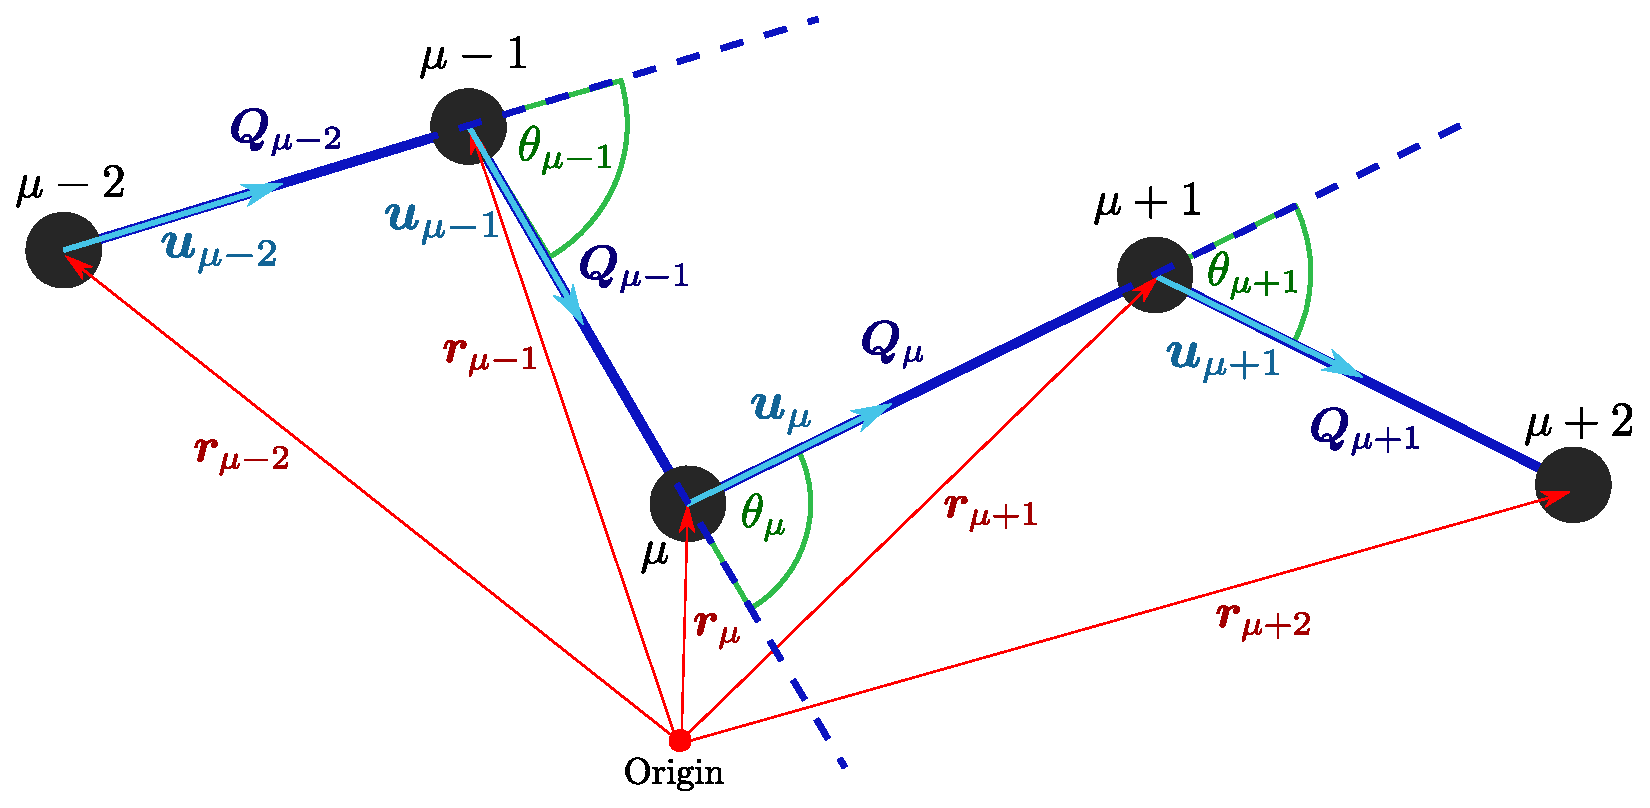
\includegraphics[width=11cm,height=!]{bending_potential_diagram.eps}
    \caption{Diagram demonstrating labelling scheme for beads, connectors and angles. $\bm{u}$ is a unit vector in the direction of the bead-to-bead vector $\bm{Q}$. Note that angle ($\theta_\mu$) numbering starts at 2, since bead 1 has no angle.}
    \label{bending_potential_diagram}
\end{figure}

We denote the bending potential by $\phi_{\mathrm{b},\mu}$, where $\phi_\mathrm{b}$ refers to the potential energy due to bending, while the $\mu$ subscript references segmental angle $\mu$. In this case we will firstly deal with a bending potential of the form \cite{Saadat2016}:
\begin{equation}
\label{bending potential}
    \phi_{\mathrm{b},\mu}/k_\mathrm{B} T = C (1-\cos{\theta_\mu})
\end{equation}
where C is a rigidity constant. 

Now consider bead $\mu$ in Fig.~\ref{bending_potential_diagram}. It has angle $\theta_\mu$ associated with it, which we can calculate by the dot product:
\begin{equation}
\label{theta definition}
    \theta_\mu = \arccos({\bm{u}_{\mu-1} \bm{\cdot} \bm{u}_{\mu}})
\end{equation}
where the unit vectors $\bm{u}_i$ can be expressed as $\bm{Q}_i/Q_i$, and the connector vectors $\bm{Q}$ can be expressed in terms of bead position vectors $\bm{r}_i$ as:
\begin{equation}
    \bm{Q}_\mu = \bm{r}_{\mu+1} - \bm{r}_{\mu}
\end{equation}

Now consider the force due to the bending potential on bead $\mu$. This will actually be a combination of the force from $\theta_\mu$, as well as adjacent angles $\theta_{\mu \pm 1}$. Specifically, we can denote the force on bead $\mu$ due to potential $\mu'$ as $\bm{F}^\mathrm{b}_{\mu, \mu'}$, and then identify the total force as:
\begin{equation}
    \bm{F}^\mathrm{b}_{\mu} = \bm{F}^\mathrm{b}_{\mu, \mu} + \bm{F}^\mathrm{b}_{\mu, \mu-1} + \bm{F}^\mathrm{b}_{\mu, \mu+1}
\end{equation}
We can further find each of these forces as a gradient of the potential (in other words, the force can be found by determining how energy changes with bead position), namely:
\begin{subequations}
\label{Forces on bead}
\begin{equation}
    \bm{F}_{\mu, \mu}^{\mathrm{b}}=-\frac{\partial \phi_{\mathrm{b}, \mu}}{\partial \bm{r}_{\mu}}=-\frac{\partial \phi_{\mathrm{b}, \mu}}{\partial \theta_{\mu}}\left\{\frac{\partial \theta_{\mu}}{\partial \bm{u}_{\mu}} \cdot \frac{\partial \bm{u}_{\mu}}{\partial \boldsymbol{r}_{\mu}}+\frac{\partial \theta_{\mu}}{\partial \bm{u}_{\mu-1}} \cdot \frac{\partial \bm{u}_{\mu-1}}{\partial \bm{r}_{\mu}}\right\}
\end{equation}
\begin{equation}
    \bm{F}_{\mu, \mu-1}^{\mathrm{b}}=-\frac{\partial \phi_{\mathrm{b}, \mu-1}}{\partial \bm{r}_{\mu}}=-\frac{\partial \phi_{\mathrm{b}, \mu-1}}{\partial \theta_{\mu-1}}\frac{\partial \theta_{\mu-1}}{\partial \bm{u}_{\mu-1}} \cdot \frac{\partial \bm{u}_{\mu-1}}{\partial \boldsymbol{r}_{\mu}}
\end{equation}
\begin{equation}
    \bm{F}_{\mu, \mu+1}^{\mathrm{b}}=-\frac{\partial \phi_{\mathrm{b}, \mu+1}}{\partial \bm{r}_{\mu}}=-\frac{\partial \phi_{\mathrm{b}, \mu+1}}{\partial \theta_{\mu+1}}\frac{\partial \theta_{\mu+1}}{\partial \bm{u}_{\mu}} \cdot \frac{\partial \bm{u}_{\mu}}{\partial \boldsymbol{r}_{\mu}}
\end{equation}
\end{subequations}
where expansions arise from application of the multivariate chain rule to Eq.~\eqref{theta definition}. 
The task now is to derive the form of the total force given a particular potential.

Firstly we can derive the parts which do not depend on the form of the potential.
We have the following results:
\begin{subequations}
\begin{equation}
    \frac{\partial \theta_{\mu}}{\partial \bm{u}_{\mu}} = \frac{\partial \arccos({\bm{u}_{\mu-1} \bm{\cdot} \bm{u}_{\mu}})}{\partial ({\bm{u}_{\mu-1} \bm{\cdot} \bm{u}_{\mu}})} \frac{\partial ({\bm{u}_{\mu-1} \bm{\cdot} \bm{u}_{\mu}})}{\partial \bm{u}_{\mu}} = -\frac{1}{\sqrt{1-\cos^2\theta_{\mu}}} \bm{u}_{\mu-1} = -\frac{1}{\sin{\theta_\mu}} \bm{u}_{\mu-1}
\end{equation}
\begin{equation}
    \frac{\partial \theta_{\mu}}{\partial \bm{u}_{\mu-1}} = -\frac{1}{\sin{\theta_\mu}} \bm{u}_{\mu}
\end{equation}
\begin{equation}
    \frac{\partial \theta_{\mu-1}}{\partial \bm{u}_{\mu-1}} = -\frac{1}{\sin{\theta_{\mu-1}}} \bm{u}_{\mu-2}
\end{equation}
\begin{equation}
    \frac{\partial \theta_{\mu+1}}{\partial \bm{u}_{\mu}} = -\frac{1}{\sin{\theta_{\mu+1}}} \bm{u}_{\mu+1}
\end{equation}
\end{subequations}
For the $\partial \bm{u} / \partial \bm{r}$ terms, this will give a symmetric tensor with different diagonal and cross terms.
To demonstrate, consider the following derivative:
\begin{subequations}
\begin{equation}
    \frac{\partial u_{\mu, x}}{\partial r_{\mu,x}} = \frac{\partial \left[ r_{\mu+1,x} - r_{\mu,x} \right] / \sqrt{(r_{\mu+1,x} - r_{\mu,x})^2 + \ldots}}{\partial r_{\mu,x}}
\end{equation}
\begin{equation}
    \frac{\partial u_{\mu, x}}{\partial r_{\mu,x}} = \frac{\partial Q_{\mu,x}/\sqrt{Q_{\mu,x}^2 + \ldots }}{\partial Q_{\mu,x}} \frac{\partial Q_{\mu,x}}{\partial r_{\mu,x}}
\end{equation}
\begin{equation}
    \frac{\partial u_{\mu, x}}{\partial r_{\mu,x}} = -1 \left[ \frac{1}{\sqrt{Q_{\mu,x}^2 + \ldots }} - \frac{Q_{\mu,x}^2}{(Q_{\mu,x}^2 + \ldots)^{3/2}} \right]
\end{equation}
\begin{equation}
    \frac{\partial u_{\mu, x}}{\partial r_{\mu,x}} = \frac{Q_{\mu,x}^2}{Q_\mu^3} - \frac{1}{Q_\mu} = \frac{1}{Q_\mu} \left( u_{\mu,x}^2 - 1\right)
\end{equation}
\end{subequations}
Similarly, the cross terms can be shown to be:
\begin{subequations}
\begin{equation}
    \frac{\partial u_{\mu, x}}{\partial r_{\mu,y}} = \frac{\partial \left[ r_{\mu+1,x} - r_{\mu,x} \right] / \sqrt{(r_{\mu+1,x} - r_{\mu,x})^2 + (r_{\mu+1,y} - r_{\mu,y})^2 +\ldots}}{\partial r_{\mu,y}}
\end{equation}
\begin{equation}
    \frac{\partial u_{\mu, x}}{\partial r_{\mu,y}} = \frac{\partial Q_{\mu,x}/\sqrt{Q_{\mu,x}^2 + Q_{\mu,y}^2 + \ldots }}{\partial Q_{\mu,y}} \frac{\partial Q_{\mu,y}}{\partial r_{\mu,y}}
\end{equation}
\begin{equation}
    \frac{\partial u_{\mu, x}}{\partial r_{\mu,y}} = \frac{Q_{\mu,x} Q_{\mu,y}}{Q_\mu^3} = \frac{1}{Q_\mu} \left( u_{\mu,x} u_{\mu,y} \right)
\end{equation}
\end{subequations}
Therefore, overall due to symmetry we have that:
\begin{equation}
    \frac{\partial \bm{u}_{\mu}}{\partial \bm{r}_\mu} = \frac{1}{Q_\mu} \left( \bm{u}_\mu \bm{u}_\mu - \bm{\delta} \right)
\end{equation}
where $\bm{\delta}$ is the diagonal unit tensor. 
Similarly, we can show that:
\begin{equation}
    \frac{\partial \bm{u}_{\mu-1}}{\partial \bm{r}_\mu} = \frac{1}{Q_{\mu-1}} \left( -\bm{u}_{\mu-1} \bm{u}_{\mu-1} + \bm{\delta} \right)
\end{equation}
We then evaluate the dot products in Eq.~\eqref{Forces on bead}. These are as follows:
\begin{subequations}
\label{dot product terms}
\begin{equation}
    \begin{split}
        \frac{\partial \theta_{\mu}}{\partial \bm{u}_{\mu}} \cdot \frac{\partial \bm{u}_{\mu}}{\partial \boldsymbol{r}_{\mu}} &= -\frac{1}{\sin{\theta_\mu}} \frac{1}{Q_\mu} \bm{u}_{\mu-1} \cdot \left( \bm{u}_\mu \bm{u}_\mu - \bm{\delta} \right) \\
        &= -\frac{1}{\sin{\theta_\mu}} \frac{1}{Q_\mu} \left( \cos{\theta_\mu} \bm{u}_\mu - \bm{u}_{\mu-1} \right)
    \end{split} 
\end{equation}
\begin{equation}
    \begin{split}
        \frac{\partial \theta_{\mu}}{\partial \bm{u}_{\mu-1}} \cdot \frac{\partial \bm{u}_{\mu-1}}{\partial \boldsymbol{r}_{\mu}} &= -\frac{1}{\sin{\theta_\mu}} \frac{1}{Q_{\mu-1}} \bm{u}_{\mu} \cdot \left( -\bm{u}_{\mu-1} \bm{u}_{\mu-1} + \bm{\delta} \right) \\
        &= -\frac{1}{\sin{\theta_\mu}} \frac{1}{Q_{\mu-1}} \left( -\cos{\theta_\mu} \bm{u}_{\mu-1} + \bm{u}_{\mu} \right)
    \end{split} 
\end{equation}
\begin{equation}
    \begin{split}
        \frac{\partial \theta_{\mu-1}}{\partial \bm{u}_{\mu-1}} \cdot \frac{\partial \bm{u}_{\mu-1}}{\partial \boldsymbol{r}_{\mu}} &= -\frac{1}{\sin{\theta_{\mu-1}}} \frac{1}{Q_{\mu-1}} \bm{u}_{\mu-2} \cdot \left( -\bm{u}_{\mu-1} \bm{u}_{\mu-1} + \bm{\delta} \right) \\
        &= -\frac{1}{\sin{\theta_{\mu-1}}} \frac{1}{Q_{\mu-1}} \left( -\cos{\theta_{\mu-1}} \bm{u}_{\mu-1} + \bm{u}_{\mu-2} \right)
    \end{split} 
\end{equation}
\begin{equation}
    \begin{split}
        \frac{\partial \theta_{\mu+1}}{\partial \bm{u}_{\mu}} \cdot \frac{\partial \bm{u}_{\mu}}{\partial \boldsymbol{r}_{\mu}} &= -\frac{1}{\sin{\theta_{\mu+1}}} \frac{1}{Q_{\mu}} \bm{u}_{\mu+1} \cdot \left( \bm{u}_{\mu} \bm{u}_{\mu} - \bm{\delta} \right) \\
        &= -\frac{1}{\sin{\theta_{\mu+1}}} \frac{1}{Q_{\mu}} \left( \cos{\theta_{\mu+1}} \bm{u}_{\mu} - \bm{u}_{\mu+1} \right)
    \end{split} 
\end{equation}
\end{subequations}

Therefore, in general we have that:
\begin{subequations}
\begin{equation}
    \bm{F}^\mathrm{b}_{\mu} = \bm{F}^\mathrm{b}_{\mu, \mu} + \bm{F}^\mathrm{b}_{\mu, \mu-1} + \bm{F}^\mathrm{b}_{\mu, \mu+1}
\end{equation}
\begin{multline}
    \bm{F}^\mathrm{b}_\mu = \frac{\partial \phi_{\mathrm{b}, \mu}}{\partial \theta_{\mu}} \frac{1}{\sin{\theta_\mu}} \left[\frac{1}{Q_\mu} \left( \cos{\theta_\mu} \bm{u}_\mu - \bm{u}_{\mu-1} \right) + \frac{1}{Q_{\mu-1}} \left( -\cos{\theta_\mu} \bm{u}_{\mu-1} + \bm{u}_{\mu} \right) \right]\\
    + \frac{\partial \phi_{\mathrm{b}, \mu-1}}{\partial \theta_{\mu-1}} \frac{1}{\sin{\theta_{\mu-1}}} \left[\frac{1}{Q_{\mu-1}} \left( -\cos{\theta_{\mu-1}} \bm{u}_{\mu-1} + \bm{u}_{\mu-2} \right) \right]  + \\
    \frac{\partial \phi_{\mathrm{b}, \mu+1}}{\partial \theta_{\mu+1}} \frac{1}{\sin{\theta_{\mu+1}}} \left[\frac{1}{Q_{\mu}} \left( \cos{\theta_{\mu+1}} \bm{u}_{\mu} - \bm{u}_{\mu+1} \right) \right] \\
\end{multline}
\end{subequations}

For our particular form of the bending potential detailed in Eq.~\eqref{bending potential}, we can see that:
\begin{equation}
    -\frac{\partial \phi_{\mathrm{b},i}}{\partial \theta_{i}} = -k_\mathrm{B} T C \sin{\theta_i}
\end{equation}
Therefore, we can see that the $\sin$ terms will cancel in Eq.~\eqref{dot product terms}, and we are left with the following equation for the force on bead $\mu$:
\begin{multline}
\label{Forces for 1-cos potential}
    \frac{\bm{F}^\mathrm{b}_\mu}{k_\mathrm{B} T C} = \left[\frac{1}{Q_\mu} \left( \cos{\theta_\mu} \bm{u}_\mu - \bm{u}_{\mu-1} \right) + \frac{1}{Q_{\mu-1}} \left( -\cos{\theta_\mu} \bm{u}_{\mu-1} + \bm{u}_{\mu} \right) \right]\\
    + \left[\frac{1}{Q_{\mu-1}} \left( -\cos{\theta_{\mu-1}} \bm{u}_{\mu-1} + \bm{u}_{\mu-2} \right) \right]  + \left[\frac{1}{Q_{\mu}} \left( \cos{\theta_{\mu+1}} \bm{u}_{\mu} - \bm{u}_{\mu+1} \right) \right] \\
\end{multline}

which is nearly, but not quite the same as Saadat and Khomami's expression... Apparently the $-\cos{\theta_{\mu-1}} \bm{u}_{\mu-1}$ term should be positive.
Given subsequent tests and 

\subsection{Alternate forms of bending potential}
One alternate form of the bending potential is described by Yamakawa \cite{Yamakawa2016} as a discrete analogue of the wormlike chain for a bead-rod model.
In this case, the bending potential is given as:
\begin{equation}
\label{bending potential discrete WLC}
    \phi_{\mathrm{b},\mu} = \frac{\alpha}{2} \theta_\mu^2
\end{equation}
where $\alpha$ is the bending force constant, which in this case is dimensional unlike the previous definition of $C$ in Eq.~\eqref{bending potential}.
This follows from the definition of the bending energy in the continuous WLC as $U = 1/2 \alpha [\partial \bm{u}(s)/\partial s]^2$, where $\bm{u}(s)$ is the chain contour as a function of path length $s$.
However, in this case the stiffness parameter $\lambda^{-1}$ (twice the persistence length) is defined as:
\begin{equation}
    \lambda^{-1}=l \frac{1+\langle\cos \theta\rangle}{1-\langle\cos \theta\rangle}
\end{equation}
where $l$ is the rod length and:
\begin{equation}
    \langle\cos {\theta}\rangle=\int_{0}^{\pi} e^{-\alpha {\theta}^{2} / 2 k_{\mathrm{B}} T} \cos {\theta} \sin {\theta} d {\theta} / \int_{0}^{\pi} e^{-\alpha {\theta}^{2} / 2 k_{\mathrm{B}} T} \sin {\theta} d {\theta}
\end{equation}
This integral should be evaluated numerically to give $\lambda$ as a function of $\alpha$, or alternatively one can solve for $\alpha$ given a particular persistence length. 
It's unclear whether the same chain statistics would be obtained if the earlier form of the bending potential given in Eq.~\eqref{bending potential} was used, with the same persistence length given by the $\cos \theta$ averages.

\subsection{Updating semi-implicit scheme to use bending potential}
Here I want to highlight the changes made to the semi-implicit scheme so that it works with the bending potential.
We follow Prakash and Prabhakar's paper \cite{Prabhakar2004}, which the code follows.
This begins with the following overall stochastic differential equation:
\begin{equation}
    \mathrm{d} \boldsymbol{R}=\left[\boldsymbol{K} \cdot \boldsymbol{R}+\frac{1}{4} \boldsymbol{D} \cdot \boldsymbol{F}^{\phi}\right] \mathrm{d} t^{*}+\frac{1}{\sqrt{2}} \boldsymbol{B} \cdot \mathrm{d} \boldsymbol{W}
\end{equation}
where $\bm{K}$ is a block matrix of flow field tensors, $\bm{R}$ is the position vector block matrix, $\bm{D}$ is the diffusion tensor block matrix, $\bm{F}^{\phi}$ is the total force on each bead due to potentials, $\bm{B}$ is a block matrix such that $\bm{B} = \bm{D} \cdot \bm{D}^{\mathrm{T}}$, and $d\bm{W}$ is a block matrix describing a random Weiner process.
In general, $\bm{F}^{\phi}$ can be split into spring forces, $\bm{F}^{\mathrm{s}}$, and other forces, which may be excluded volume, bending or torsional potentials, external forces etc.
We'll denote these other forces by $\bm{F}^{\mathrm{O}}$.
Now in step 1 of the semi-implicit solution, we get a halfway step of the position vectors as follows:
\begin{equation}
    \tilde{\boldsymbol{R}}_{n+1}=\boldsymbol{R}_{n}+\left[\boldsymbol{K} \cdot \boldsymbol{R}_{n}+\frac{1}{4} \boldsymbol{D}_{n} \cdot \boldsymbol{F}_{n}^{\mathrm{S}}+\frac{1}{4} \boldsymbol{D}_{n} \cdot \boldsymbol{F}_{n}^{\mathrm{O}}\right] \Delta t^{*}+\frac{1}{\sqrt{2}} \Delta \boldsymbol{S}_{n}
\end{equation}
Where we have replaced $\boldsymbol{F}_{n}^{\mathrm{E}}$ in the original by $\boldsymbol{F}_{n}^{\mathrm{O}}$ to denote the additional bending potential forces, rather than simply the excluded volume forces.
The basic principle is then to construct a semi-implicit solution to this equation, where we must construct the following term made up of all the explicit parts of the equation:
\begin{multline}
    \tilde{\boldsymbol{\Upsilon}}_{n+1}=\boldsymbol{R}_{n} \\
    +\left[\frac{1}{2}\left\{\boldsymbol{K} \cdot \boldsymbol{R}_{n}+\boldsymbol{K} \cdot \tilde{\boldsymbol{R}}_{n+1}\right\}  +\frac{1}{8} \boldsymbol{D}_{n} \cdot \boldsymbol{F}_{n}^{\mathrm{S}}+\frac{1}{8} \boldsymbol{D}_{n} \cdot\left\{\boldsymbol{F}_{n}^{\mathrm{O}}+\tilde{\boldsymbol{F}}_{n+1}^{\mathrm{O}}\right\}\right] \Delta t^{*} \\
     + \frac{1}{\sqrt{2}} \Delta \boldsymbol{S}_{n}
\end{multline}
Previously, the code was using the total force $\bm{F}^{\phi}$ for the $1/8 \boldsymbol{D}_{n} \cdot \boldsymbol{F}_{n}^{\mathrm{S}}$ and $1/8 \boldsymbol{D}_{n} \cdot \boldsymbol{F}_{n}^{\mathrm{E}}$ parts, but was not adding in the additional contribution from the bending potential to the predictor step contribution $1/8 \boldsymbol{D}_{n} \cdot \tilde{\boldsymbol{F}}_{n+1}^{\mathrm{O}}$. 
Once this was added in, the bending potential seems to be working correctly!

\subsection{Tests to check code}
Here I'll list the tests I've written to check that the code works. These are divided into two sections. The unit tests basically check some edge cases for the bending potential function itself and ensure the results for some low-bead cases are what we expect, while the validation tests essentially check that the average angles match the expected distribution for an actual BD simulation.

\subsubsection{Unit tests}
\begin{enumerate}

    \item the force is zero for the two-bead case
    
\noindent This one is straightforward, for the $N_\mathrm{beads} = 2$ case there are no bending potentials and hence we should get zero bending force.

    \item no bending potential gives no force
    
\noindent Also straightforward, I have an option for no bending potential.

    \item The force should be zero when the beads are co-linear
    
\noindent When the beads are co-linear, we have that all $\theta = \pi$, meaning that the potential should be zero and there should be no force. This is implemented by a chain of 5 beads arranged along the x-axis, then checking the force is zero.

    \item For a 3-bead chain, we should be able to check the forces by hand
    
\noindent Here I'm running two tests. The first is with the three beads, with the two connector vectors perpendicular to each other:
\begin{align*}
    \bm{r}_1 &= \{ 0, 1, 0 \} \\
    \bm{r}_2 &= \{ 0, 0, 0 \} \\
    \bm{r}_3 &= \{ 1, 0, 0 \}
\end{align*}
which for a $1-\cos(\theta)$ bending potential, should give the forces (as per Eq.~\eqref{Forces for 1-cos potential}):
\begin{align*}
    \bm{F}_1 &= \{ -1, 0, 0 \} \\
    \bm{F}_2 &= \{ 1, 1, 0 \} \\
    \bm{F}_3 &= \{ 0, -1, 0 \}
\end{align*}
Note that these forces are aligned such that the force vector is perpendicular to the connector unit vector $\bm{u}$ for the end beads. 
This is generally true for the end-beads of a chain, since this direction of movement gives the fastest rate of change of the angle, and hence is the line of steepest decent for the bending potential (which defines the direction of the force). 

I'll also test a second case with the connector vectors $30^{\circ}$ apart:
\begin{align*}
    \bm{r}_1 &= \{ -\sqrt{3}/2, 1/2, 0 \} \\
    \bm{r}_2 &= \{ 0, 0, 0 \} \\
    \bm{r}_3 &= \{ 1, 0, 0 \}
\end{align*}
which for a $1-\cos(\theta)$ bending potential, should give the forces (as per Eq.~\eqref{Forces for 1-cos potential}):
\begin{align*}
    \bm{F}_1 &= \{ -1/4, -\sqrt{3}/4, 0 \} \\
    \bm{F}_2 &= \{ 1/4, (2+\sqrt{3})/4, 0 \} \\
    \bm{F}_3 &= \{ 0, -1/2, 0 \}
\end{align*}
Once again, the end bead forces are perpendicular to the connector vector. 
This also provides a reasonable test of the final bead force equation, since we can compare our geometric intuition with the algebraic equation.

    \item For a 4-bead chain, we can compare a simple case with the calculated result
    
\noindent We have the following bead positions:
\begin{align*}
    \bm{r}_1 &= \{ 0, 0, 0 \} \\
    \bm{r}_2 &= \{ 1, 0, 0 \} \\
    \bm{r}_3 &= \{ 1, -1, 0 \} \\
    \bm{r}_4 &= \{ 1+\sqrt{2}/2, -1 + \sqrt{2}/2, 0 \}
\end{align*}
This is the same as the following diagram, where all connector vector lengths are equal to $1$:

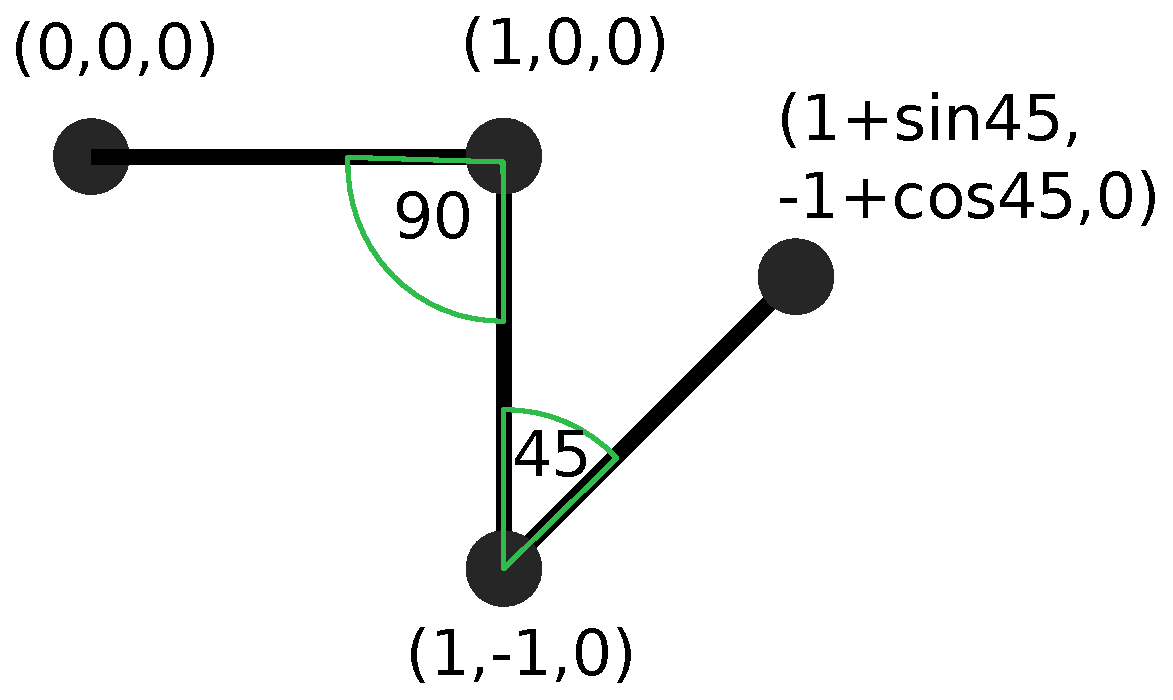
\includegraphics[width=5cm,height=!]{4_beads_example.eps}

which for a $1-\cos(\theta)$ bending potential, should give the forces (as per Eq.~\eqref{Forces for 1-cos potential}):
\begin{align*}
    \bm{F}_1 &= \{ 0, 1, 0 \} \\
    \bm{F}_2 &= \{ -1-\sqrt{2}/2, -1, 0 \} \\
    \bm{F}_3 &= \{ (1+\sqrt{2})/2, 1/2, 0 \} \\
    \bm{F}_4 &= \{ 1/2, -(2+\sqrt{2})/2, 0 \}
\end{align*}

    \item For a 5-bead chain, we can compare a simple case with the calculated result
    
\noindent We have the following bead positions:
\begin{align*}
    \bm{r}_1 &= \{ 0, 0, 0 \} \\
    \bm{r}_2 &= \{ \sqrt{2}/2, \sqrt{2}/2, 0 \} \\
    \bm{r}_3 &= \{ \sqrt{2}/2+1, \sqrt{2}/2, 0 \} \\
    \bm{r}_4 &= \{ \sqrt{2}/2+1+\sqrt{3}/2, \sqrt{2}/2+1/2, 0 \} \\
    \bm{r}_5 &= \{ \sqrt{2}/2+1+\sqrt{3}, \sqrt{2}/2, 0 \}
\end{align*}
This is the same as the following diagram, where all connector vector lengths are equal to $1$:

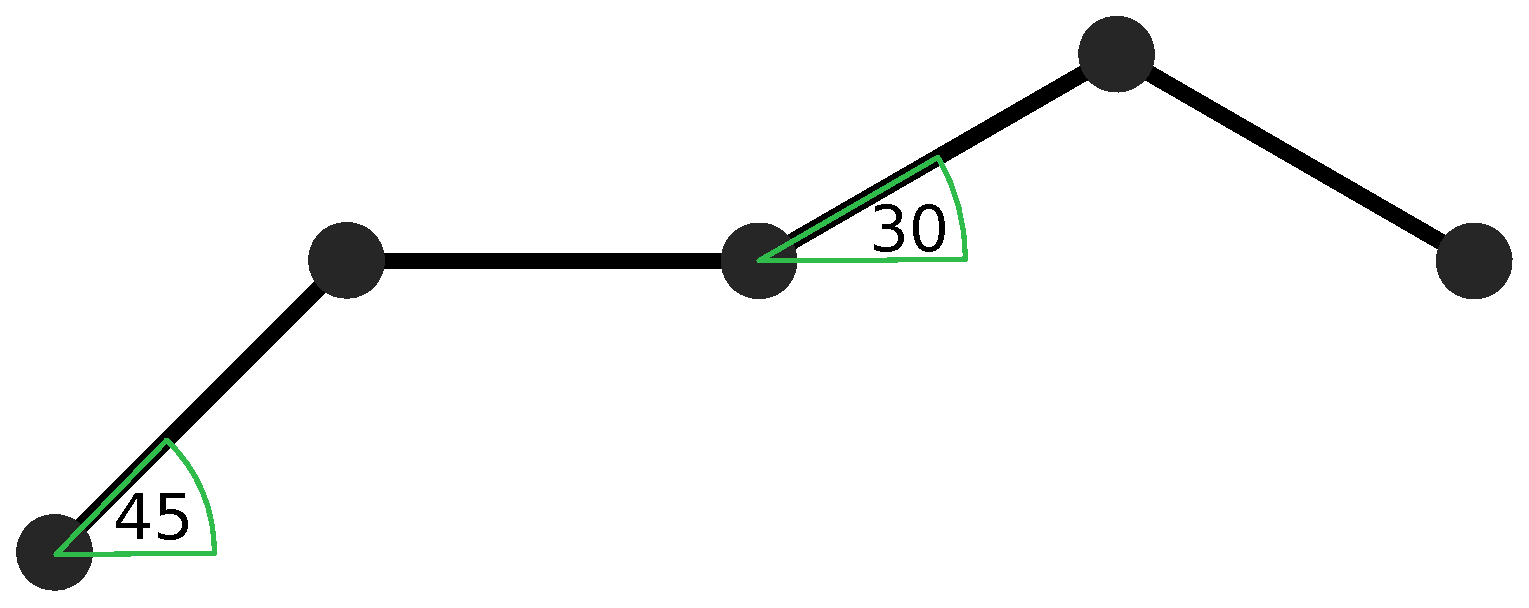
\includegraphics[width=5cm,height=!]{5_beads_example.eps}

which for a $1-\cos(\theta)$ bending potential, should give the forces (as per Eq.~\eqref{Forces for 1-cos potential}):
\begin{align*}
    \bm{F}_1 &= \{ -1/2, 1/2, 0 \} \\
    \bm{F}_2 &= \{ 1/2, -\sqrt{2}/2-1, 0 \} \\
    \bm{F}_3 &= \{ -1/4-\sqrt{3}/4, 5/4+\sqrt{3}/4+\sqrt{2}/2, 0 \} \\
    \bm{F}_4 &= \{ 1/4, -3/2-\sqrt{3}/4, 0 \} \\
    \bm{F}_5 &= \{ \sqrt{3}/4, 3/4, 0 \}
\end{align*}

    \item Finally, a randomly generated initial condition and result was created on MATLAB, and then checked against the Fortran result as an additional check for both 4-bead and 5-bead cases. This should cover $>5$ bead cases as well, as we only want to check inner beads.

\end{enumerate}

\subsubsection{Validation tests}
\begin{enumerate}

    \item Compare with expected vector-vector correlation for a wormlike chain
    
\noindent This one is straightforward, for the $N_\mathrm{beads} = 2$ case there are no bending potentials and hence we should get zero bending force.

    \item For a Rouse chain with bending potential, compare with analytical result for angular distribution
    
\noindent In general we can express the angular distribution as the sum of the spring force law and the bending potential:
\begin{equation}
    \phi = \frac{1}{2} H \sum^{N-1}_{k} \bm{Q}_k^2 + \sum^{N-2}_k C ( 1 - \bm{u}_k \cdot \bm{u}_{k+1} )
\end{equation}
% Does the $\bm{Q}_k^2$ refer to $\bm{Q}_k \cdot \bm{Q}_k$? 
% This seems to make sense as the potential should be a scalar as it is an energy, not a vector or tensor. 
This would mean that we can write out the equilibrium configurational distribution function as:
\begin{equation}
    \psi_{\mathrm{eq}}(\bm{Q}^{N-1}) = \frac{e^{-\phi/k_\mathrm{B} T}}{\int e^{-\phi/k_\mathrm{B} T} d\bm{Q}^{N-1} }
\end{equation}
So that then we have the following integral for a 3-bead chain:
\begin{equation}
    \int \int \int \int e^{- H/2k_\mathrm{B} T Q_1^2 \bm{u}_1 \cdot \bm{u}_1} e^{- H/2k_\mathrm{B} T Q_2^2 \bm{u}_2 \cdot \bm{u}_2} e^{-C/k_\mathrm{B} T (1 - \bm{u}_1 \cdot \bm{u}_2)} dQ_1 dQ_2 d\bm{u}_1 d\bm{u}_2
\end{equation}
There are two things we can do to simplify this equation. 
Firstly, we note that $\bm{u}_i \cdot \bm{u}_i = 1$, since the dot product of a unit vector with itself must be the scalar $1$. 
This allows us to separate the spring integral parts of the expression from the part which depends upon the angle between the beads. 
This is in general true as long as the spring force law depends purely upon the spring length and not orientation. 
The second simplification is to orient our co-ordinate system along $\bm{u}_1$, such that $\theta \equiv \bm{u}_1 \cdot \bm{u}_2$ is the polar angle in spherical co-ordinates. 
The result is that when we take an average which depends only on the angle $\theta$ between the springs, we can greatly simplify the resulting expression:
\begin{align}
    \langle \cos \theta \rangle &= \frac{\int_{Q_1} \int_{Q_2} e^{- H/2k_\mathrm{B} T (Q_1^2 + Q_2^2)} dQ_1 dQ_2 \int_{\theta} \int_{\beta} \cos \theta e^{-\phi_\mathrm{b}/k_\mathrm{B} T}  d\theta d\beta}{\int_{Q_1} \int_{Q_2} e^{- H/2k_\mathrm{B} T (Q_1^2 + Q_2^2)} dQ_1 dQ_2 \int_{\theta} \int_{\beta}  e^{-\phi_\mathrm{b}/k_\mathrm{B} T} d\theta d\beta} \\
    &= \frac{\int_\theta \sin{\theta} \cos{\theta} e^{-\phi_\mathrm{b}/k_\mathrm{B} T} d\theta}{\int_\theta \sin{\theta} e^{-\phi_\mathrm{b}/k_\mathrm{B} T} d\theta}
\end{align}
where $\beta$ is the azimuthal angle and $\theta$ runs from $0$ to $\pi$.
For our current bending potential of $\phi_{\mathrm{b}}/k_\mathrm{B} T = C (1-\cos{\theta})$, we have that (from mathematica):
\begin{align}
    \langle \cos \theta \rangle &= \frac{-1 + C + \left(C+1\right) e^{-2C}}{C\left(1-e^{-2C}\right)} \\
    &= -\frac{1}{C} + \coth(C)
\end{align}
Furthermore, we can integrate out the other factors to obtain the distribution in $\theta$, which gives us:
\begin{equation}
    \psi_{eq}(\theta) = \frac{ \sin{\theta}  e^{-\phi_\mathrm{b}/k_\mathrm{B} T}}{\int_\theta \sin{\theta} e^{-\phi_\mathrm{b}/k_\mathrm{B} T} d\theta} = \left[\frac{C}{1-e^{-2 C}}\right] \sin{\theta} e^{-\frac{C}{k_\mathrm{B}T}\left(1-\cos{\theta}\right)}
\end{equation}
Therefore, we should expect the distribution of angles for our trimer at equilibrium to follow this distribution. 

Fig.~\ref{C curves no HI 3 beads} gives an example of this correct distribution function. Additionally, we can see from Fig.~\ref{Bending dist FF 10 beads HI} that although not proven here, for a 10-bead chain with HI and a FENE-Fraenkel spring potential ($H^*_R = 200$, $\delta Q^*_R = 0.1$), the average bending angle still follows exactly the same distribution.
\begin{figure}[!ht]
    \centering
    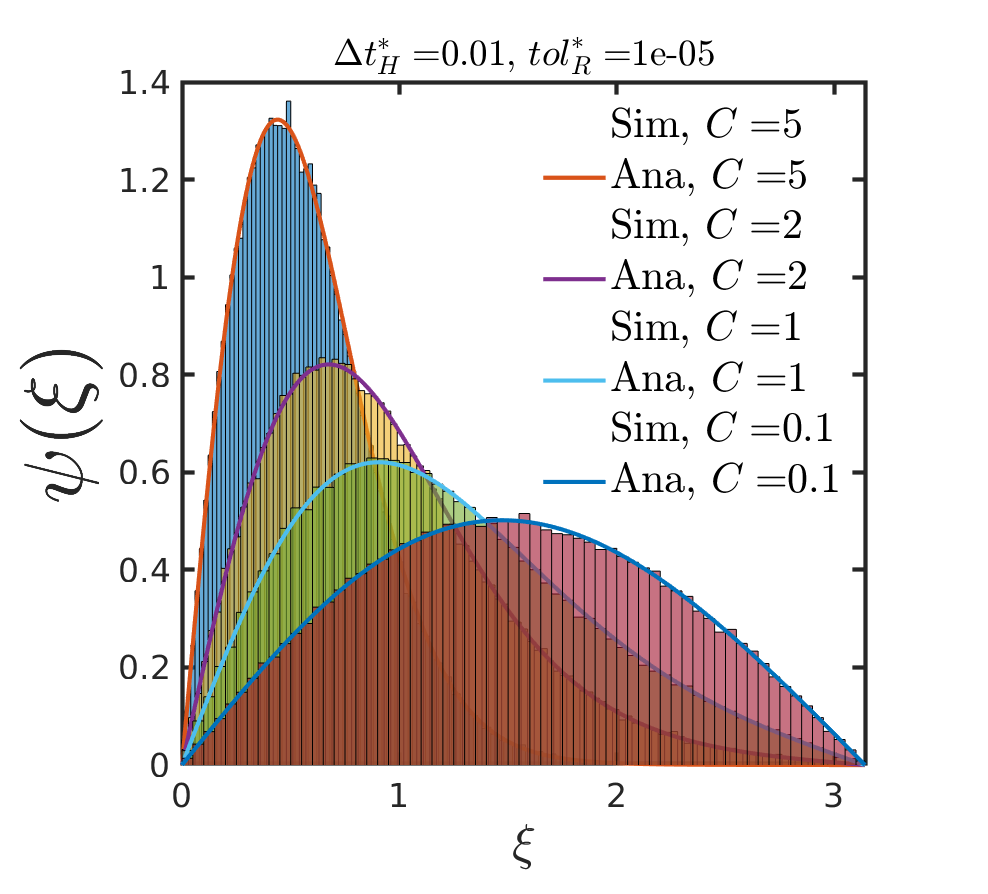
\includegraphics[width=8cm,height=!]{C_curves.eps}
    \caption{Comparison of analytical and simulated bending angles $\xi$ against bending stiffness value $C$.}
    \label{C curves no HI 3 beads}
\end{figure}

\begin{figure}[!ht]
    \centering
    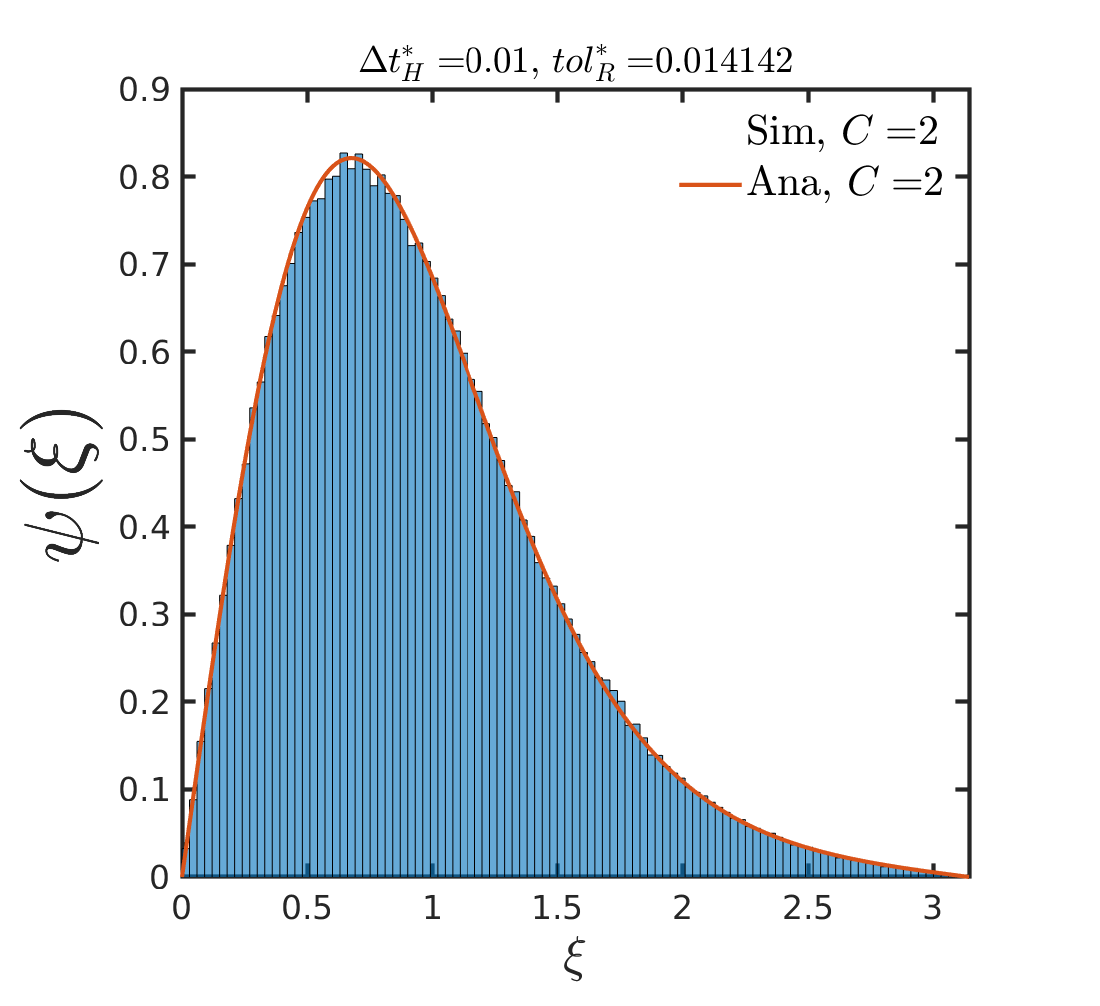
\includegraphics[width=8cm,height=!]{Bending_dist_10_beads_FF_HI.eps}
    \caption{FENE-Frankel spring 10-bead chain with HI and a bending potential. FENE-Fraenkel spring parameters are $H^*_R = 200$, $\delta Q^*_R = 0.1$.}
    \label{Bending dist FF 10 beads HI}
\end{figure}

\end{enumerate}

\section{Hydrodynamic Interaction}

\subsection{RPY tensor}

\subsection{Fixman's solution method implementation}

\section{Sampling and data output}

\subsection{Stress tensor calculation}

\subsection{Netcdf files}

\section{Semi-implict predictor-corrector}

\subsection{Cubic equation solvers}

\subsection{Lookup tables}

\section{List of inputs}

\section{Post-processing files}

\printbibliography

\end{document}
